\documentclass[UTF8,a4paper,11pt]{ctexart}

\usepackage[margin=1in]{geometry}
\usepackage{amsmath,amssymb,amsfonts,bm}
\usepackage{booktabs,multirow,array,tabularx}
\usepackage{graphicx}
\usepackage{float}
\usepackage{caption}
\usepackage{subcaption}
\usepackage{pgfplots}
\pgfplotsset{compat=1.18}
\captionsetup[figure]{font=small,labelfont=bf}
\captionsetup[table]{font=small,labelfont=bf}
\usepackage{hyperref}
\usepackage{xcolor}
\usepackage{enumitem}

\hypersetup{
    colorlinks=true,
    linkcolor=blue,
    citecolor=blue,
    urlcolor=blue
}

\newcommand{\R}{\mathbb{R}}
\newcommand{\DeltaW}{\Delta W}
\newcommand{\Wzero}{W_0}
\newcommand{\rank}{\operatorname{rank}}

\title{TiRA：面向高秩参数高效微调的一种分块化高秩适配方法研究}
\author{}
\date{}

\makeatletter
\let\ps@plain\ps@empty
\makeatother

\begin{document}
\pagestyle{empty}
\maketitle

\begin{abstract}
预训练大语言模型具备强大的通用语言能力，但在复杂下游任务中仍需进行任务特定适配。全参数微调通常计算开销较大，且对显存资源需求较高；相比之下，参数高效微调方法通过优化少量额外引入的参数，实现了训练成本的显著降低。其中，LoRA 通过低秩分解实现高效适配，但其有效秩受预设参数 $r$ 的限制，在复杂场景中可能出现秩不足问题。针对这一局限，本文提出分块化高秩适配方法 TiRA，将权重增量矩阵划分为 $M\times M$ 个子块，并构造 $K$ 组低维向量对；每组包含 $M$ 对向量，分别通过外积生成 $M$ 个子块，再沿一条错位块对角线填充至权重增量矩阵中。TiRA 在保持与 LoRA 相同可训练参数量的前提下，通过重新组织权重增量矩阵中的可训练参数，使权重更新突破 LoRA 的全局低秩约束，并具有更高的秩上界。谱分析进一步显示，相比 LoRA，TiRA 训练后的权重增量通常具有更高的实测有效秩和更分散的谱能量分布。此外，该方法仍然保持与原始权重可合并的特性，因此在推理阶段不引入额外开销。本文在常识推理、开放域对话生成和数学推理三类任务上对该方法进行了系统评估。实验结果表明，在同等可训练参数预算设置下，TiRA 在 Llama-2-7B 与 Llama-3-8B 等模型上取得优异的性能。特别是在后者的 GSM8K 数学推理任务上，达到 $72.86\%$ 的准确率，较 LoRA 提升 $6.97$ 个百分点，较 HiRA 提升 $2.05$ 个百分点。本文代码与实验数据已公开于 \url{https://github.com/loop-xxx/TiRA}。
\end{abstract}

\section{引言}

预训练大语言模型具备强大的通用语言能力，但其原始参数通常难以直接适配特定下游任务。全参数微调可以有效提升任务性能，却面临高昂的显存与计算开销。随着模型规模持续增大，如何在有限计算资源下实现高效、稳定的任务适配，已成为大语言模型落地应用中的重要问题。

为缓解全参数微调的资源压力，已有大量研究转向参数高效微调。这类方法通常冻结预训练模型主体参数，仅引入并训练少量额外参数，从而显著降低微调成本。其中，以 LoRA\cite{hu2022lora} 为代表的基于重参数化的方法直接建模网络内部线性层的任务特定权重增量；该方法的低秩权重增量可在推理阶段与基础权重合并，因此已成为当前参数高效微调研究中的重要范式。

然而，LoRA 的核心假设是权重增量具有低秩结构。该设计适用于相对简单的任务适配，但在复杂推理或生成任务中，固定秩 $r$ 所张成的低维更新子空间可能不足以刻画任务所需的高维权重变化，从而限制模型适配能力。直接提高适配秩虽然能够扩大更新空间，但也会同步增加可训练参数量、显存占用和优化成本，削弱参数高效微调的效率优势。

围绕 LoRA 的上述局限，已有方法从不同角度进行扩展。AdaLoRA\cite{zhang2023adalora} 采用类奇异值分解形式参数化权重增量，并依据不同权重矩阵的重要性动态分配秩预算，从而缓解原方法对各层、各模块均匀分配固定秩所带来的次优问题；但该方法本质上仍是在低秩适配框架内重新分配秩资源，难以从结构上突破低秩更新空间的表达限制。DoRA\cite{liu2024dora} 将预训练权重分解为幅度和方向两个部分，并分别建模二者在微调过程中的变化，使低秩适配能够更接近全参数微调中的权重变化模式；但其方向分量仍沿用低秩更新方式，对更新空间维度的扩展有限。MoRA\cite{jiang2024mora} 关注低秩更新对知识学习和记忆能力的限制，通过方阵适配器并结合非参数降维与升维算子，在相近参数量下提高更新矩阵的秩；不过，静态映射函数的引入也使适配权重与原始权重的直接合并更加复杂。HiRA\cite{huang2025hira} 利用 Hadamard 积构造高秩适配形式，将低秩矩阵 $BA$ 与冻结的预训练权重 $W_0$ 逐元素相乘，从而在一定条件下提高权重增量的秩上界；但其高秩结构依赖于预训练权重本身，更新形式仍受到原始权重结构的约束。RandLoRA\cite{albert2025randlora} 进一步尝试在参数高效约束下实现满秩更新，通过固定的随机低秩基矩阵及其可训练缩放系数组合构造权重增量，从而缓解低秩适配的秩不足问题；但由于主要更新方向由非可训练随机基预先给定，其表达能力仍受到随机基覆盖范围的影响。由此可见，现有方法仍难以同时满足不增加可训练参数量、显著提高权重更新的秩上界、保持更新结构充分可训练以及在推理阶段易于合并这几方面需求。

因此，本文关注如下问题：在保持与 LoRA 相同可训练参数预算、并保留权重可合并特性的前提下，能否通过重新组织权重增量矩阵中的可训练参数，突破 LoRA 的全局低秩约束，并形成更适合复杂任务的更新结构？

于是，本文提出一种分块化高秩适配方法（Tiled Rank-1 Subblock Adaptation for High-Rank Parameter-Efficient Fine-Tuning, TiRA）。该方法不再对整个权重增量矩阵进行全局低秩分解，而是将权重增量矩阵 $\DeltaW$ 划分为 $M\times M$ 个块网格，并将可训练参数组织为 $K$ 个适配组。每组通过 $M$ 对低维向量的外积，在块网格的一条错位块对角线上生成 $M$ 个秩为 1 的子块，如图~\ref{fig:lora_tira} 所示。该设计使每组构成秩上限为 $M$ 的子矩阵，而 $K$ 组叠加后的增量矩阵秩上限可达 $KM$。当设置 $K=M=r$ 时，TiRA 的参数量为 $r(d_{\mathrm{out}}+d_{\mathrm{in}})$，与 LoRA 完全一致，却可将权重更新的秩上界从 $r$ 提升至 $r^2$，实现同等参数预算下的平方级秩上界扩展。

\begin{figure}[H]
    \centering
    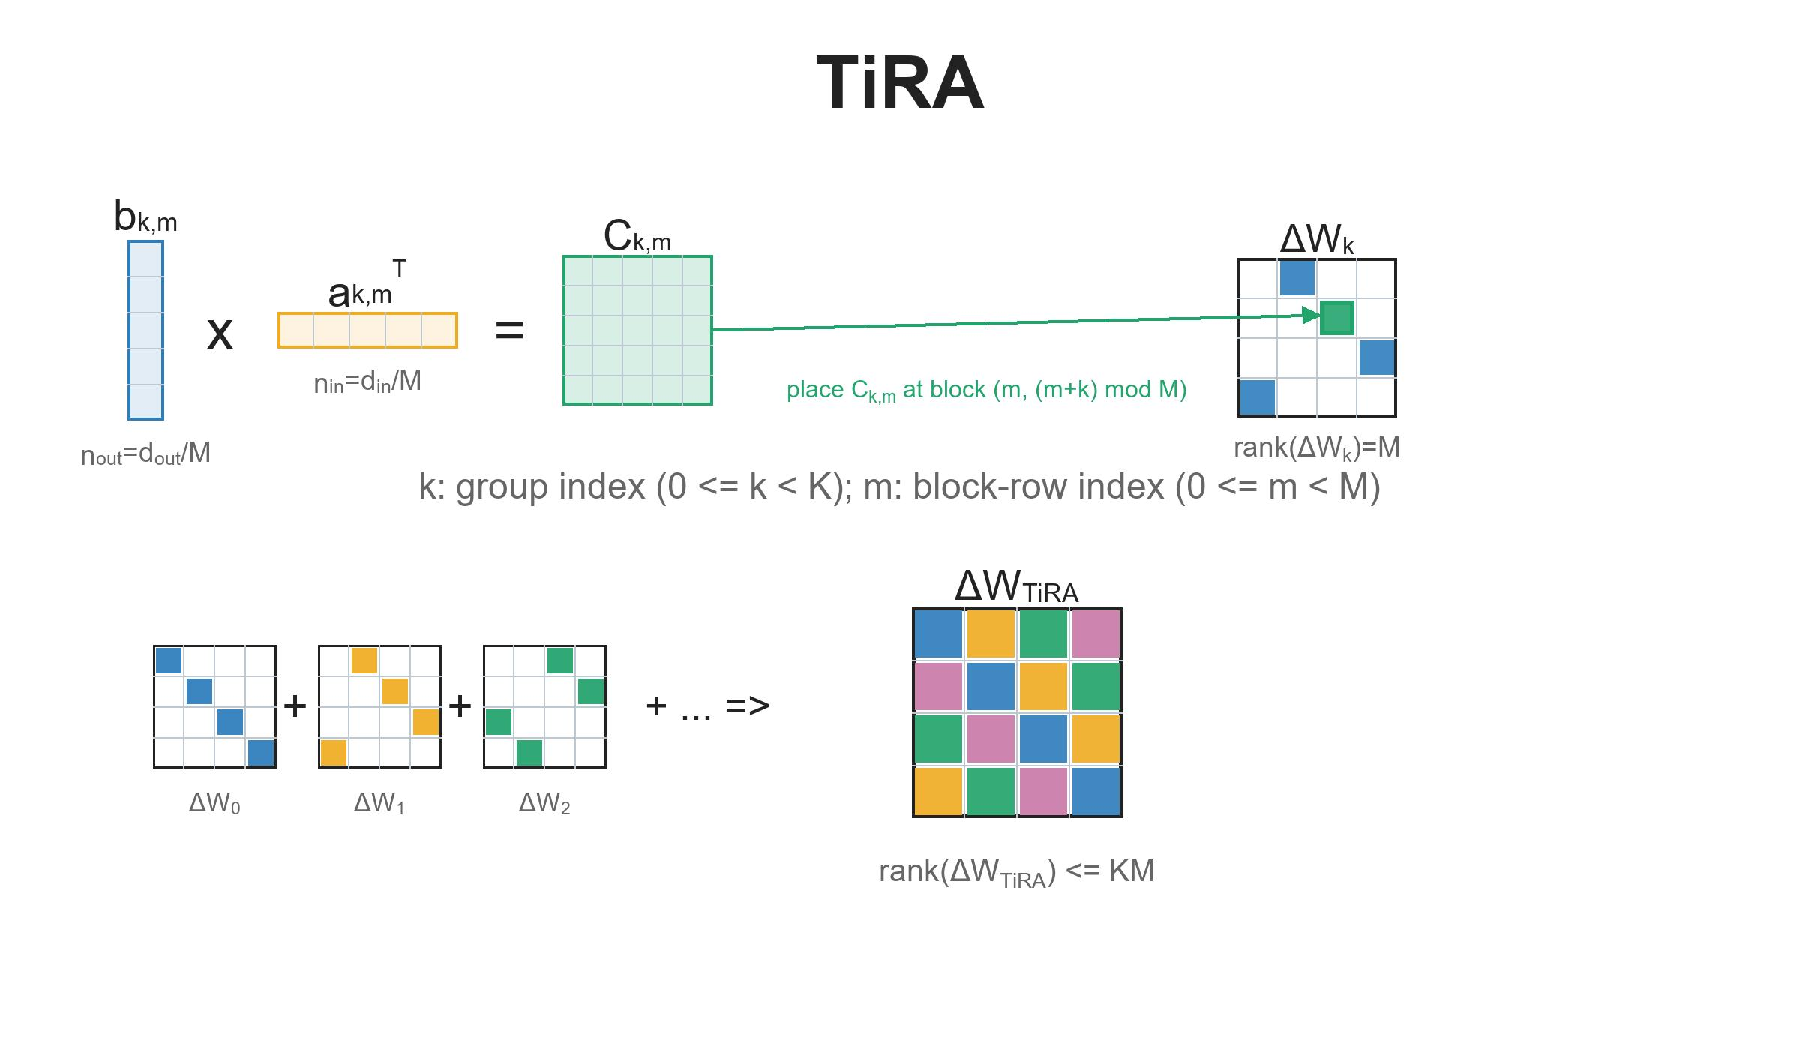
\includegraphics[width=0.96\linewidth]{figures/tira_architecture.pdf}
    \caption{TiRA 的分块填充机制示意图。图中展示第 $k$ 组适配器的子块生成与填充过程：每对可训练低维向量经外积运算得到秩为 1 的子块 $C_{k,m}$，并放置于块位置 $(m,(m+k)\bmod M)$。多个错位块对角分组叠加后形成完整权重增量 $\Delta W_{\mathrm{TiRA}}$，其秩上限为 $KM$。其中 $K$ 与 $M$ 分别控制参数分组数与分块粒度。}
    \label{fig:lora_tira}
\end{figure}

多步数学推理任务通常要求模型进行较长链条的中间推导，其复杂度随推理深度显著增加。为进一步验证复杂任务对适配秩的需求，本文在 GSM8K\cite{cobbe2021gsm8k} 训练集上按答案长度构建 Easy 与 Challenge 两个难度子集，答案越长通常对应更长的推理链和更高的推理难度。在此基础上，本文将各子集按 $9:1$ 划分训练集与验证集，并进行 LoRA 秩对比实验，实验超参数见附录~\ref{app:lora_hyperparams}。结果如图~\ref{fig:rank_motivation} 所示。Easy 子集准确率在较低秩区间快速提升，由 $r=8$ 时的 $56.80\%$ 提升至 $r=32$ 时的 $67.47\%$，随后随秩进一步增大出现轻微回落（$r=128$ 时降至 $65.07\%$），呈现早期饱和与高秩冗余特征。相比之下，Challenge 子集在低秩区间提升较为有限，$r=8$、$r=16$ 与 $r=32$ 时均为 $42.90\%$，但在更高秩设置下继续上升，最终在 $r=128$ 时达到 $47.45\%$。需要指出的是，改变 LoRA rank 会同时改变可训练参数量，因此该实验主要说明复杂任务对更高维更新空间和更大适配容量存在需求，而不能单独证明在固定参数预算下提高秩上限一定有效。

为进一步闭合这一动机链，本文在后续分块粒度实验中采用同等参数预算设置进行验证。具体而言，在 Qwen-2-1.5B 上固定 $K=32$，使 TiRA 与 LoRA（$r=32$）具有相同可训练参数量，并仅改变分块粒度 $M$。实验结果显示，LoRA（$r=32$）的 GSM8K 准确率为 $68.08\%$，而 TiRA 在 $M=2$、$M=4$ 和 $M=8$ 时分别达到 $68.16\%$、$68.39\%$ 和 $68.84\%$。这表明，在参数预算保持一致的情况下，通过分块结构提高权重更新的秩上限仍能够带来性能增益。相关结果将在表~\ref{tab:ablation} 和图~\ref{fig:ablation_m_trend} 中进一步分析。

\begin{figure}[H]
    \centering
    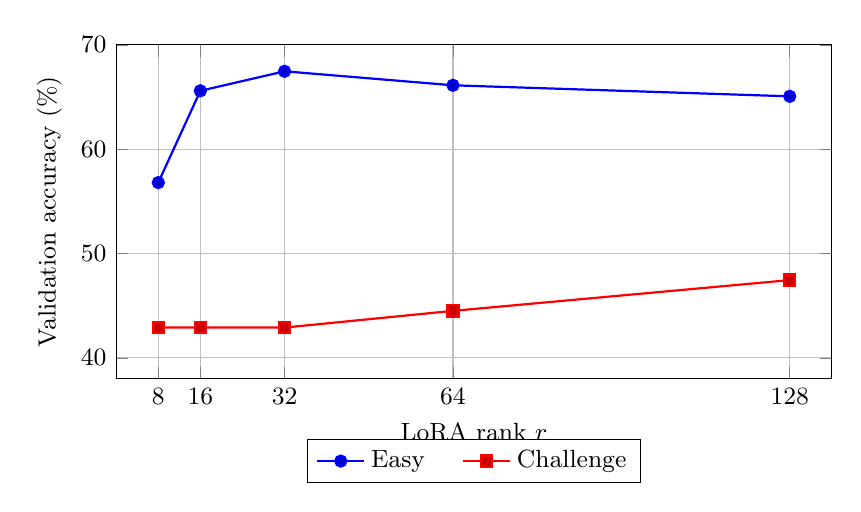
\begin{tikzpicture}
    \begin{axis}[
        width=0.88\linewidth,
        height=0.48\linewidth,
        xlabel={LoRA rank $r$},
        ylabel={Validation accuracy (\%)},
        xmin=0, xmax=136,
        ymin=38, ymax=70,
        xtick={8,16,32,64,128},
        grid=both,
        tick label style={font=\small},
        label style={font=\small},
        legend style={
            at={(0.5,-0.18)},
            anchor=north,
            legend columns=2,
            font=\small,
            /tikz/every even column/.append style={column sep=0.4cm}
        },
    ]
    \addplot+[blue, thick, mark=*] coordinates {
        (8,56.80) (16,65.60) (32,67.47) (64,66.13) (128,65.07)
    };
    \addplot+[red, thick, mark=square*] coordinates {
        (8,42.90) (16,42.90) (32,42.90) (64,44.50) (128,47.45)
    };
    \legend{Easy, Challenge}
    \end{axis}
    \end{tikzpicture}
    \caption{Qwen-2-1.5B 模型在不同 LoRA 秩 $r$ 下于 GSM8K Easy 与 Challenge 子集微调后的验证准确率变化。横轴为 LoRA 秩，纵轴为验证集准确率（\%）。}
    \label{fig:rank_motivation}
\end{figure}

本文的主要贡献如下：
\begin{enumerate}[leftmargin=2em]
    \item 提出 TiRA，一种面向大语言模型的高秩参数高效适配方法。该方法在严格保持与 LoRA 同等参数预算的前提下，通过重新组织权重增量矩阵中的可训练参数，使权重更新突破全局低秩约束，并获得更高的秩上界。
    \item 提出 TiRA 的超参数解耦配置策略，并系统分析最优分块粒度与模型规模之间的关系。本文将分组数 $K$ 与分块粒度 $M$ 解耦，使参数预算和高秩结构可独立调节；进一步的实验表明，最优 $M$ 通常随模型规模增大而右移，同时过高的分块粒度可能引发秩过载效应。
    \item 通过多类下游任务实验验证 TiRA 的有效性。实验结果表明，TiRA 在保持参数高效性和无额外推理开销的同时，在常识推理、开放域对话生成和数学推理任务上均优于现有代表性 PEFT 方法。
\end{enumerate}

\section{相关工作}

\subsection{LoRA 及其扩展方法}

LoRA\cite{hu2022lora} 是基于重参数化的参数高效微调代表方法，其核心思想是在冻结预训练权重的同时，以可训练低秩旁路建模线性层的任务特定权重增量。围绕这一范式，已有研究主要沿两类路线展开。第一类方法在低秩适配框架内提升参数利用效率或更新质量，例如 AdaLoRA\cite{zhang2023adalora} 根据参数重要性动态分配秩预算，以提升固定参数预算下的利用效率；DoRA\cite{liu2024dora} 则从幅度和方向两个部分建模权重变化，使低秩适配更接近全参数微调的更新模式。第二类方法直接关注低秩更新空间受限的问题，包括通过方阵适配器提高更新秩的 MoRA\cite{jiang2024mora}、利用 Hadamard 积构造高秩更新的 HiRA\cite{huang2025hira}，以及借助随机基矩阵实现满秩更新的 RandLoRA\cite{albert2025randlora}。

上述方法从不同角度增强了适配的表达能力或训练效率，但在更新秩、可训练自由度、权重可合并性和实现复杂度之间仍存在权衡。本文提出的 TiRA 属于高秩重参数化适配方法，其重点不是重新分配低秩预算或依赖外部随机基，而是在保持与 LoRA 同等参数预算和可合并特性的同时，通过结构化分块构造显式地提高权重增量的秩上界。

\subsection{其他 PEFT 方法}

除重参数化方法外，提示类适配也是参数高效微调的重要方向。该类方法通过在输入层或隐藏层中引入可训练虚拟令牌，并在冻结预训练主干参数的条件下诱导模型产生任务特定行为。代表性方法包括 Prefix Tuning\cite{li2021prefix}、Prompt Tuning\cite{lester2021power} 和 P-Tuning v2\cite{xiao2022ptuning}。与直接修改网络内部线性投影的 LoRA 及其变体不同，提示类方法主要通过调整输入或中间表示空间实现适配，其性能通常受提示长度、初始化方式和任务形式影响较大。本文方法属于重参数化路线，因此后续实验主要选取 LoRA 及其高秩扩展方法作为重点对比对象。

\section{方法}

\subsection{旁路适配框架}

基于重参数化的参数高效微调方法通常作用于神经网络中的线性投影模块。鉴于 Transformer\cite{vaswani2017attention} 已成为当前大语言模型的主流架构，其内部的 Query、Key、Value、Output 投影矩阵以及前馈网络的投影层均为线性投影，因此这些模块构成了重参数化适配的主要应用对象。该类方法冻结预训练网络的全部权重参数，仅在线性投影层旁引入少量可训练旁路参数，用于建模任务特定权重增量。对于原始权重矩阵 $W\in\R^{d_{\mathrm{out}}\times d_{\mathrm{in}}}$，该类方法学习任务特定权重增量 $\DeltaW$，并以
\begin{equation}
    W_{\mathrm{task}} = W + \DeltaW
\end{equation}
的形式对原线性投影进行增量调整。该设计在部署阶段较为便利，微调完成后，旁路参数可通过矩阵加法与原权重合并，从而在推理阶段不引入额外计算延迟或显存开销。

\subsection{权重增量构造形式}

TiRA 继承上述重参数化旁路适配框架，并通过分块化构造突破全局低秩约束。其将增量矩阵 $\DeltaW\in\R^{d_{\mathrm{out}}\times d_{\mathrm{in}}}$ 划分为 $M\times M$ 个单元块；每个块的尺寸为 $n_{\mathrm{out}}\times n_{\mathrm{in}}$，其中 $n_{\mathrm{out}}=d_{\mathrm{out}}/M$，$n_{\mathrm{in}}=d_{\mathrm{in}}/M$；同时为每个块分配独立的秩为 1 的适配器。

具体而言，TiRA 将秩为 1 的适配器划分为 $K$ 组。第 $k$ 组（$0\leq k<K$）包含 $M$ 对可训练低维向量
\begin{equation}
    \{\bm{b}_{k,m},\bm{a}_{k,m}\}_{m=0}^{M-1},\quad
    \bm{b}_{k,m}\in\R^{n_{\mathrm{out}}},\quad
    \bm{a}_{k,m}\in\R^{n_{\mathrm{in}}}
\end{equation}
每对低维向量通过外积运算生成一个秩为 1 的子块：
\begin{equation}
    C_{k,m}=\bm{b}_{k,m}\bm{a}_{k,m}^{\top}\in\R^{n_{\mathrm{out}}\times n_{\mathrm{in}}}
\end{equation}
TiRA 采用错位块对角分组策略构造完整增量矩阵。第 $k$ 组适配器占据一条错位块对角线，其中第 $m$ 个秩为 1 的子块放置于第 $m$ 行、第 $(m+k)\bmod M$ 列，其余块位置置零。由此可定义第 $k$ 组稀疏增量矩阵 $\Delta W_k$：
\begin{equation}
    [\Delta W_k]_{i,j}=
    \begin{cases}
        C_{k,m}, & i=m,\; j=(m+k)\bmod M,\\
        0, & \text{otherwise}
    \end{cases}
\end{equation}
$K$ 组叠加后得到总权重增量：
\begin{equation}
    \DeltaW = \sum_{k=0}^{K-1}\Delta W_k
\end{equation}
当 $K=M$ 时，$M$ 条错位块对角线刚好覆盖全部 $M\times M$ 个块位置，每个块位置由一个低维向量外积生成的秩为 1 的子块填充。为直观说明错位块对角分组策略，附录~\ref{app:k3m3} 给出了 $K=M=3$ 时 TiRA 增量矩阵的具体构造示例。

在初始化方面，TiRA 沿用 LoRA 中常见的非对称初始化策略。具体而言，$\bm{a}_{k,m}$ 采用 Kaiming uniform 初始化\cite{he2015rectifier}，$\bm{b}_{k,m}$ 初始化为零。由于每个子块由 $C_{k,m}=\bm{b}_{k,m}\bm{a}_{k,m}^{\top}$ 给出，零初始化 $\bm{b}_{k,m}$ 可使训练开始时所有子块均为零，从而保证初始权重增量 $\DeltaW=0$，模型初始行为与原始预训练模型保持一致。同时，非零初始化的 $\bm{a}_{k,m}$ 可为 $\bm{b}_{k,m}$ 提供有效梯度方向，避免完全零初始化导致的对称性问题。

\subsection{参数量与秩分析}

TiRA 的参数量可由适配组数直接得到。每个适配组包含 $M$ 个秩为 1 的子块，每个子块由一对长度分别为 $n_{\mathrm{out}}$ 和 $n_{\mathrm{in}}$ 的低维向量生成，因此单个适配组的参数量为 $M(n_{\mathrm{out}}+n_{\mathrm{in}})=d_{\mathrm{out}}+d_{\mathrm{in}}$。对于 $K$ 个适配组，TiRA 的总参数量为
\begin{equation}
    \mathrm{Params}=K\times M\times(n_{\mathrm{out}}+n_{\mathrm{in}})=K(d_{\mathrm{out}}+d_{\mathrm{in}})
\end{equation}
因此，当设置 $K=M=r$ 时，TiRA 与秩为 $r$ 的 LoRA 具有相同的可训练参数量，均为 $r(d_{\mathrm{out}}+d_{\mathrm{in}})$。在这一相同预算下，二者的差异主要体现在参数组织方式上：LoRA 将参数组织为两个全局低秩因子矩阵，其权重增量整体受秩 $r$ 约束；TiRA 则将同等数量的参数分配到分块矩阵的不同位置，并在每个块内构造秩为 1 的局部更新。此时，错位块对角结构使这些局部更新覆盖全部 $M\times M$ 个块位置，多个局部低秩更新在全局矩阵中组合后，可使权重更新的全局秩上界达到 $r^2$。

\subsection{超参数解耦设计}

TiRA 对超参数 $K$ 与 $M$ 进行解耦设计：$M$ 主要决定分块粒度，$K$ 主要决定实际参数量和块内秩上界。这种解耦使得 TiRA 能够在不改变分块结构的情况下，通过调整 $K$ 灵活匹配不同计算预算。具体而言，在固定分块粒度 $M$ 的条件下，调整 $K$ 可以改变可训练参数量，并通过改变每个块位置上的叠加层数 $L=K/M$ 调节块内秩上界。为使所有 $M$ 条斜带被均匀使用，$K$ 应满足 $K\geq M$ 且为 $M$ 的整数倍，即
\begin{equation}
    K=L\cdot M,
\end{equation}
其中 $L\in\mathbb{Z}^{+}$ 表示每个块位置上的叠加层数。当 $L=1$（即 $K=M$）时，每条斜带对应一组适配器；当 $L\geq2$ 时，进入多层叠加模式，参数量、块内秩以及总秩上限随 $L$ 扩展。若固定 $M$ 并在计算资源允许的情况下提高块内秩上界，可将 $K$ 设置为 $M$ 的倍数（如 $K=2M,3M,\ldots$）。此时第 $k$ 组仍遵循循环移位对角规则放置秩为 1 的子块，但同一斜带位置由 $L$ 组参数产生的秩为 1 的子块求和累加。附录~\ref{app:m3k6} 给出了 $M=3,K=6$（$L=2$）时的构造示例。

在该构造下，每个单元块内包含 $L$ 个独立低维向量外积之和，块内秩上界由 1 提升至 $L$。因此，总秩上界为
\begin{equation}
    \rank(\DeltaW)\leq \min\{M^2L,\;d_{\mathrm{out}},\;d_{\mathrm{in}}\}
\end{equation}
可见，当 $M$ 固定时，增大 $L$ 可通过多层叠加提升块内秩上界，并使总秩上界近似随 $L$ 线性增长。

特别地，当 $M=1$ 时，TiRA 不再对权重增量矩阵进行分块，此时 $L=K$，$\DeltaW$ 由 $K$ 个秩为 1 的外积矩阵叠加而成，结构等价于低秩分解 $\DeltaW=BA$，其中 $B\in\R^{d_{\mathrm{out}}\times K}$ 由 $\{\bm{b}_k\}$ 按列拼接而成，$A\in\R^{K\times d_{\mathrm{in}}}$ 由 $\{\bm{a}_k^{\top}\}$ 按行拼接而成。

\subsection{分块结构的作用}

为避免将全局秩上界误解为任意高秩矩阵的完全覆盖，本节进一步明确 TiRA 可表示的权重更新形式。LoRA 将权重增量写作 $\DeltaW=BA$，因此在秩参数为 $r$ 时，它可以表示所有全局秩不超过 $r$ 的矩阵。TiRA 的约束则作用在分块结构上。设 $K=L\cdot M$，并将 $\DeltaW$ 按 $M\times M$ 划分为子块 $\{\Delta W_{i,j}\}_{i,j=0}^{M-1}$。根据错位块对角填充规则，位置 $(i,j)$ 上的子块只由满足 $k\equiv j-i \pmod M$ 的适配组写入，因此每个子块至多由 $L$ 个秩为 1 的外积叠加得到，即
\begin{equation}
    \rank(\Delta W_{i,j})\leq L.
\end{equation}
反过来，任意满足上述块内秩约束的分块矩阵，都可以对每个子块分别进行至多 $L$ 项秩为 1 的分解，并放入对应的错位块对角组中来表示。由此可将 TiRA 的可表示范围写为
\begin{equation}
    \mathcal{T}_{M,L}=\{\DeltaW:\rank(\Delta W_{i,j})\leq L,\;0\leq i,j<M\}.
\end{equation}
因此，TiRA 表示的是块内低秩的分块更新，而不是所有全局秩不超过 $KM$ 的矩阵。若某个权重增量矩阵存在 $\rank(\Delta W_{i,j})>L$ 的子块，即使其全局秩并不高，也不能由当前 $K=L\cdot M$ 的 TiRA 精确表示。特别地，在 $K=M=r$ 的同等参数预算下，TiRA 的每个子块均受秩为 1 的约束；其全局秩上界可以达到 $r^2$，但并不覆盖全部秩不超过 $r^2$ 的矩阵。

上述限制也正是 TiRA 的结构先验来源。LoRA 假设任务相关扰动可以由少量全局方向共同解释，因而适合更新集中在少数主方向上的情形；TiRA 则假设更新可以拆解为多个输入通道块与输出通道块之间的局部简单交互。块内低秩约束降低了单个局部交互的复杂度，避免每个块独立学习过于自由的高维变换；错位块对角填充则使每个适配组在所有块行和块列中各写入一次，从而让有限参数覆盖更分散的通道块组合，而不是只作用于主对角块或少数固定位置。当 $K=M$ 时，所有块位置均被覆盖；当 $K=L\cdot M$ 时，每个块位置由 $L$ 个局部秩为 1 的分量叠加，块内秩上界随之提高。因此，TiRA 通过这种“局部低秩、全局分散”的参数组织方式，为权重增量提供了不同于 LoRA 全局低秩分解的结构选择；该先验是否有效，取决于它是否匹配下游任务所需要的权重更新模式，并将在后续实验中加以验证。

\section{实验}

为全面评估 TiRA 在复杂任务上的适配能力，本文在常识推理、开放域对话生成和数学推理三类下游任务上开展实验。

\subsection{数据集}

常识推理实验遵循 LLM-Adapters\cite{hu2023llmadapters} 的设置。本文将八项常识推理数据集合并为统一训练集，并从中随机抽取 120 条样本构成验证集，共计使用 170,420 条问答样本进行微调。这些子任务涵盖 BoolQ\cite{bisk2019boolq}、PIQA\cite{bisk2020piqa}、SIQA\cite{sap2019socialiqa}、HellaSwag\cite{zellers2019hellaswag}、WinoGrande\cite{sakaguchi2021winogrande}、ARC-e、ARC-c\cite{clark2018arc} 和 OBQA\cite{mihaylov2018openbookqa}，分别覆盖布尔型问答、物理与社会常识推理、常识自然语言推理、代词消解、科学选择题以及开放书本式多步推理等能力。

开放域对话生成实验基于 ConvAI2\cite{dinan2019convai2} 数据集展开。该数据集为每段多轮对话提供历史上下文和角色人设，其中人设通常由 4--5 句描述性文本构成。遵循既有设置，本文仅向模型提供当前说话者自身的人设描述，而不引入对话对手的角色信息；这一设置用于评估其在有限身份信息下结合上下文生成一致、自然回复的能力。

数学推理实验选用 MetaMath\cite{yu2024metamath} 作为训练语料，并在 GSM8K\cite{cobbe2021gsm8k} 原始测试集上进行评估。前者通过对 GSM8K 与 MATH 等数据进行面向推理的增强重写构建，能够提供更丰富的多步推理样本；后者由小学数学应用题组成，要求模型通过逐步推导得到最终数值答案，因此常用于衡量大语言模型的数学推理与泛化能力。

\subsection{实验设置}

\paragraph{评估指标。}
常识推理任务以准确率作为评价指标。模型首先根据输入查询生成自由文本回复，随后通过关键词匹配从中提取预测答案。对于每个样本，首个匹配到的有效关键词被视为预测结果；若未检测到目标关键词，则判定为错误。开放域对话生成任务采用 BLEU\cite{papineni2002bleu}、METEOR\cite{banerjee2005meteor}、ROUGE-L\cite{lin2004rouge} 和 BERTScore\cite{zhang2019bertscore} 等自动指标评估生成质量。数学推理任务同样采用准确率作为评价指标。具体而言，本文同时抽取生成文本中的最后一个数值和显式答案提示之后的数值，并分别与标准答案比较；若任一结果匹配，则判定该样本回答正确。

\paragraph{基线方法。}
为全面验证 TiRA 的有效性，本文选取参数高效微调领域的代表性方法作为对比基线，涵盖提示微调与重参数化适配两类技术路线。前者包括 Prompt Tuning 和 P-Tuning，后者包括 LoRA、DoRA、MoRA 和 HiRA。所有主要实验均在 Llama-2-7B\cite{touvron2023llama2} 与 Llama-3-8B\cite{grattafiori2024llama3} 两款开源大语言模型上完成。除本文复现的 TiRA 结果及分块粒度分析中的 LoRA 对照外，其余主要基线结果沿用 HiRA 的公开报告，以保证与既有工作的可比性。

\paragraph{实现细节。}
为保证实验结果与既有研究具有可比性，本文沿用 HiRA 的主要训练配置，并仅根据任务类型调整学习率。所有实验均采用 AdamW 优化器，预热步数设为 100。其中，常识推理任务以学习率 $2\times10^{-4}$ 微调 2 个 epoch，并每 80 步进行一次验证集评估以筛选最优检查点；开放域对话生成任务采用学习率 $2\times10^{-5}$ 训练 1 个 epoch；数学推理任务则以学习率 $4\times10^{-5}$ 训练 2 个 epoch。TiRA 的适配层施加于注意力模块的 Query、Key、Value 投影矩阵，以及前馈网络的上投影和下投影层。详细超参数见附录~\ref{app:tira_hyperparams}。为确保与 LoRA、DoRA、MoRA 和 HiRA 等基线公平比较，本文严格控制可训练参数量处于同一量级。

\subsection{常识推理实验结果}

\begin{table}[H]
\centering
\caption{以 Llama-2-7B 为基座模型时，各参数高效微调方法在常识推理数据集上的准确率对比。除 TiRA 外，其余基线结果引自 HiRA。最优结果以粗体标示，次优结果以下划线标示。}
\label{tab:commonsense_llama2}
\setlength{\tabcolsep}{3pt}
\makebox[\textwidth][c]{%
\footnotesize
\begin{tabular}{@{}lcccccccccc@{}}
\toprule
Method & Params (\%) & BoolQ & PIQA & SIQA & ARC-c & ARC-e & OBQA & HellaS & WinoG & Avg \\
\midrule
Prompt Tuning & 0.0012 & 55.93 & 12.35 & 30.50 & 6.06 & 8.63 & 9.40 & 6.91 & 40.57 & 21.29 \\
P-Tuning & 0.7428 & 58.75 & 36.02 & 0.20 & 0.17 & 1.98 & 0.80 & 0.01 & 0.00 & 12.24 \\
LoRA ($r=32$) & 0.8256 & 69.80 & 79.90 & 79.50 & 64.70 & 79.80 & 81.00 & 82.60 & 82.60 & 77.61 \\
DoRA ($r=32$) & 0.8256 & \underline{71.80} & \textbf{83.70} & 76.00 & 68.20 & 83.70 & 82.40 & \textbf{89.10} & 82.60 & 79.69 \\
MoRA ($r=32$) & 0.8241 & \textbf{72.17} & 80.79 & \underline{79.53} & 71.42 & 85.31 & 81.20 & 29.09 & 80.19 & 72.46 \\
HiRA ($r=32$) & 0.8256 & 71.22 & 83.35 & \underline{79.53} & \textbf{73.81} & \underline{86.74} & \textbf{84.60} & 88.12 & \underline{83.98} & \underline{81.42} \\
TiRA ($K=M=32$) & 0.8256 & 70.86 & \underline{83.62} & \textbf{80.71} & \underline{72.95} & \textbf{87.67} & \underline{84.40} & \underline{88.98} & \textbf{84.61} & \textbf{81.72} \\
\bottomrule
\end{tabular}
}
\end{table}

\begin{table}[H]
\centering
\caption{以 Llama-3-8B 为基座模型时，各参数高效微调方法在常识推理数据集上的准确率对比。除 TiRA 外，其余基线结果引自 HiRA。最优结果以粗体标示，次优结果以下划线标示。}
\label{tab:commonsense_llama3}
\setlength{\tabcolsep}{3pt}
\makebox[\textwidth][c]{%
\footnotesize
\begin{tabular}{@{}lcccccccccc@{}}
\toprule
Method & Params (\%) & BoolQ & PIQA & SIQA & ARC-c & ARC-e & OBQA & HellaS & WinoG & Avg \\
\midrule
Prompt Tuning & 0.0010 & 56.85 & 45.05 & 36.13 & 31.57 & 32.74 & 29.20 & 14.01 & 50.12 & 36.96 \\
P-Tuning & 0.6240 & 59.97 & 11.64 & 8.19 & 7.42 & 8.63 & 9.60 & 1.77 & 37.65 & 18.11 \\
LoRA ($r=32$) & 0.7002 & 70.80 & 85.20 & 79.90 & 71.20 & 84.20 & 79.00 & 91.70 & 84.30 & 80.79 \\
DoRA ($r=32$) & 0.7002 & 74.60 & 89.30 & 79.90 & 80.40 & 90.50 & 85.80 & \underline{95.50} & 85.60 & 85.20 \\
MoRA ($r=32$) & 0.6997 & 74.28 & 87.43 & 80.71 & 79.61 & 91.16 & 85.60 & 43.53 & 86.74 & 78.63 \\
HiRA ($r=32$) & 0.7002 & \underline{75.40} & \textbf{89.70} & \underline{81.15} & \underline{82.90} & \underline{93.27} & \underline{88.32} & 95.36 & \underline{87.70} & \underline{86.72} \\
TiRA ($K=M=32$) & 0.7002 & \textbf{75.66} & \underline{89.66} & \textbf{83.16} & \textbf{83.70} & \textbf{93.64} & \textbf{90.00} & \textbf{95.83} & \textbf{89.11} & \textbf{87.60} \\
\bottomrule
\end{tabular}
}
\end{table}

表~\ref{tab:commonsense_llama2} 和表~\ref{tab:commonsense_llama3} 展示了不同方法在常识推理任务上的整体表现。总体来看，TiRA 在两个基座模型上均取得最高平均准确率，体现出较为稳定的适配优势。具体而言，在 Llama-2-7B 上，该方法的平均准确率为 $81.72\%$，较 HiRA（$81.42\%$）和 DoRA（$79.69\%$）分别提升 $0.30$ 和 $2.03$ 个百分点；在 Llama-3-8B 上，其平均准确率进一步达到 $87.60\%$，相比 HiRA（$86.72\%$）和 DoRA（$85.20\%$）分别提升 $0.88$ 和 $2.40$ 个百分点。

从细分任务看，TiRA 在多数基准上保持领先。尤其在 Llama-3-8B 设置下，其在 SIQA、ARC-c、ARC-e、OBQA、HellaSwag 和 WinoGrande 等任务中均取得最优结果。上述现象表明，在相同可训练参数量约束下，TiRA 在常识推理任务中具有更强的适配能力；结合其分块化高秩结构，这一优势进一步说明，分块高秩更新结构可能更适合该类复杂推理任务的参数更新需求。

\subsection{开放域对话生成实验结果}

\begin{table}[H]
\centering
\caption{以 Llama-3-8B 为基座模型时，各参数高效微调方法在 ConvAI2 开放域对话生成数据集上的性能对比。除 TiRA 外，其余基线结果引自 HiRA。最优结果以粗体标示，次优结果以下划线标示。}
\label{tab:dialogue}
\setlength{\tabcolsep}{4pt}
\makebox[\textwidth][c]{%
\footnotesize
\begin{tabular}{@{}lcccccccc@{}}
\toprule
Method & Params (\%) & BLEU & BERT F1 & BERT-R & BERT-P & METEOR & R-L & Avg \\
\midrule
Prompt Tuning & 0.0010 & 1.45 & 82.99 & 82.99 & 83.05 & 14.72 & 13.13 & 46.39 \\
P-Tuning & 0.6240 & 1.50 & 81.52 & 81.07 & 82.01 & \underline{15.49} & 13.55 & 45.86 \\
MoRA ($r=32$) & 0.6997 & 1.60 & 84.22 & 84.06 & 84.43 & 12.37 & 11.19 & 46.31 \\
LoRA ($r=32$) & 0.7002 & 2.26 & 84.32 & 84.00 & 84.67 & 12.51 & 11.77 & 46.59 \\
DoRA ($r=32$) & 0.7002 & 2.29 & 84.32 & 84.06 & 84.62 & 12.63 & 11.78 & 46.62 \\
HiRA ($r=32$) & 0.7002 & \underline{3.41} & \textbf{84.81} & \underline{84.40} & \textbf{85.25} & 14.87 & \underline{14.05} & \underline{47.80} \\
TiRA ($K=M=32$) & 0.7002 & \textbf{3.50} & \underline{84.78} & \textbf{84.48} & \underline{85.11} & \textbf{15.66} & \textbf{14.34} & \textbf{48.04} \\
\bottomrule
\end{tabular}
}
\end{table}

表~\ref{tab:dialogue} 给出了 ConvAI2 上的开放域对话生成结果。可以看到，TiRA 在 Llama-3-8B 上取得最高平均得分，达到 $48.04\%$，分别高于 HiRA（$47.80\%$）、DoRA（$46.62\%$）、LoRA（$46.59\%$）和 MoRA（$46.31\%$）。从单项指标来看，该方法在 BLEU、BERT-R、METEOR 和 ROUGE-L 上均排名第一，在 BERT F1 与 BERT-P 上也接近最优。上述结果表明，分块化高秩适配在开放域对话生成任务中同样具有良好的适配效果，能够更好地建模角色信息与历史上下文之间的语义关联，从而提升生成回复与参考回复的一致性。

\subsection{数学推理实验结果}

\begin{table}[H]
\centering
\caption{以 Llama-3-8B 为基座模型时，各参数高效微调方法在数学推理任务上的准确率对比。训练语料为 MetaMath，测试基准为 GSM8K。除 TiRA 外，其余基线结果引自 HiRA。最优结果以粗体标示，次优结果以下划线标示。}
\label{tab:math}
\setlength{\tabcolsep}{6pt}
\makebox[\textwidth][c]{%
\footnotesize
\begin{tabular}{@{}lcc@{}}
\toprule
Method & Trainable (\%) & GSM8K \\
\midrule
Prompt Tuning & 0.0012 & 15.62 \\
P-Tuning & 0.7428 & 2.65 \\
LoRA ($r=32$) & 0.7002 & 65.89 \\
DoRA ($r=32$) & 0.7002 & 66.12 \\
MoRA ($r=32$) & 0.6997 & 67.98 \\
HiRA ($r=32$) & 0.7002 & \underline{70.81} \\
TiRA ($K=M=32$) & 0.7002 & \textbf{72.86} \\
\bottomrule
\end{tabular}
}
\end{table}

表~\ref{tab:math} 给出了 MetaMath 训练、GSM8K 测试下的数学推理结果。其中，TiRA 在 Llama-3-8B 上取得 $72.86\%$ 的准确率，为表中最优。相较于次优的 HiRA（$70.81\%$），该方法提升 $2.05$ 个百分点；与 LoRA（$65.89\%$）和 DoRA（$66.12\%$）相比，其增益分别为 $6.97$ 和 $6.74$ 个百分点。上述结果说明，在相同可训练参数预算下，分块化高秩适配能够更有效地支持复杂多步推理任务的模型微调。

\subsection{适配权重的谱分析}

为进一步从参数空间刻画 TiRA 权重更新的高秩特征，本文对数学推理实验中训练完成的适配权重增量 $\DeltaW$ 进行奇异值分解，并将其与同等参数预算下的 LoRA 进行比较。具体而言，本文选取 Llama-3-8B 在 MetaMath 上训练得到的最优检查点，分别构造 LoRA 的权重增量 $\DeltaW=BA$ 和 TiRA 的分块化权重增量，并在所有适配层及目标线性模块上统计平均谱指标。本文报告有效秩、能量秩和稳定秩三类指标。有效秩由奇异值阈值 $\tau=0.005$ 确定，用于衡量显著奇异方向的数量；能量秩表示累计平方奇异值能量达到给定比例所需的最小秩，本文分别统计 95\% 和 99\% 两种阈值。该指标越高，说明谱能量分布越分散，权重更新涉及的适配方向越多。稳定秩定义为 $\|\DeltaW\|_F^2/\|\DeltaW\|_2^2$，可视为由谱能量支撑的连续型秩度量；当能量主要集中于少数主方向时，其取值较低，而当能量分布在更多奇异方向上时，其取值相应增大。

\begin{table}[H]
\centering
\small
\caption{训练后适配权重增量 $\DeltaW$ 的谱分析结果。所有指标均在 Llama-3-8B 的 32 层及目标模块上取平均。}
\label{tab:delta_spectrum}
\begin{tabular}{lcccc}
\toprule
Method & Eff. rank & Stable rank & 95\% energy rank & 99\% energy rank \\
\midrule
LoRA ($r=32$) & 32.00 & 2.50 & 13.55 & 23.93 \\
TiRA ($M=16,K=32$) & 432.96 & 10.15 & 161.94 & 304.45 \\
TiRA ($M=32,K=32$) & \textbf{757.27} & \textbf{14.71} & \textbf{356.52} & \textbf{631.81} \\
\bottomrule
\end{tabular}
\end{table}

表~\ref{tab:delta_spectrum} 给出了训练后权重增量的总体谱指标。LoRA 的有效秩受设定秩 $r=32$ 限制，且谱能量较为集中，其 95\% 能量秩仅为 13.55。相比之下，在相同可训练参数量下，TiRA 的 $\DeltaW$ 呈现出更高的有效秩和更分散的能量分布。以 $M=32,K=32$ 为例，该方法的平均有效秩达到 757.27，95\% 能量秩达到 356.52，分别约为 LoRA 的 23.7 倍和 26.3 倍；稳定秩也由后者的 2.50 提升至 14.71。上述结果说明，分块化结构不仅提高了理论秩上界，也能在实际训练中形成更高维的权重更新子空间。

\begin{figure}[H]
    \centering
    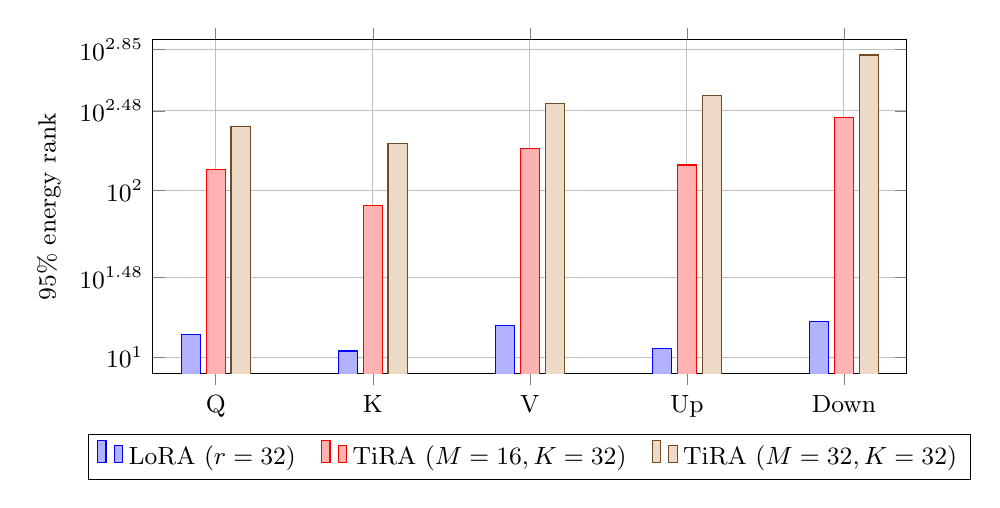
\begin{tikzpicture}
    \begin{axis}[
        ybar,
        ymode=log,
        width=0.92\linewidth,
        height=0.48\linewidth,
        bar width=7pt,
        ylabel={95\% energy rank},
        symbolic x coords={Q,K,V,Up,Down},
        xtick=data,
        ymin=8,
        ymax=800,
        ytick={10,30,100,300,700},
        grid=both,
        tick label style={font=\small},
        label style={font=\small},
        legend style={
            at={(0.5,-0.18)},
            anchor=north,
            legend columns=3,
            font=\small,
            /tikz/every even column/.append style={column sep=0.25cm}
        },
    ]
    \addplot coordinates {(Q,13.63) (K,10.91) (V,15.47) (Up,11.28) (Down,16.47)};
    \addlegendentry{LoRA ($r=32$)}
    \addplot coordinates {(Q,133.41) (K,81.53) (V,177.88) (Up,142.06) (Down,274.81)};
    \addlegendentry{TiRA ($M=16,K=32$)}
    \addplot coordinates {(Q,242.16) (K,191.69) (V,330.38) (Up,370.41) (Down,647.97)};
    \addlegendentry{TiRA ($M=32,K=32$)}
    \end{axis}
    \end{tikzpicture}
    \caption{不同目标模块上训练后 $\DeltaW$ 的 95\% 能量秩对比。纵轴采用对数尺度以展示不同方法之间的数量级差异。}
    \label{fig:delta_spectrum_rank95}
\end{figure}

图~\ref{fig:delta_spectrum_rank95} 进一步展示了不同模块上的谱分布差异。结果显示，TiRA 在 Query、Key、Value 投影以及前馈网络的上投影和下投影模块上均取得显著高于 LoRA 的 95\% 能量秩。这表明，高秩更新并非集中于个别层或个别模块，而是较稳定地存在于模型的主要线性投影模块中。其中，下投影和上投影模块的提升尤为明显，说明该方法能够在前馈网络中引入更丰富的任务相关扰动方向。上述谱分析说明 TiRA 训练后形成了更分散的更新方向，这与其在数学推理任务上的性能提升相互印证。

\subsection{分块粒度 $M$ 对适配性能的影响}

当 $M=1$ 时，TiRA 不再进行分块，其结构退化为秩为 $K$ 的低秩分解 $BA$，与 LoRA 形式等价。为分析分块粒度 $M$ 对适配性能的影响，实验固定 $K=32$，使该方法的可训练参数量与 LoRA（$r=32$）严格对齐，并仅改变分块数 $M$。为进一步考察不同模型规模下的粒度选择规律，本文选取 Qwen-2-0.5B、Qwen-2-1.5B 和 Qwen-2.5-3B\cite{yang2024qwen2,yang2024qwen25} 三个规模递进的开源模型作为主对照序列，统一在 MetaMath 上微调 2 个 epoch，并在 GSM8K 测试集上评估。详细超参数见附录~\ref{app:ablation_hyperparams}。实验结果如表~\ref{tab:ablation} 和图~\ref{fig:ablation_m_trend} 所示，表中还纳入更大规模的 Llama-3-8B，用于补充观察该规律在更大模型上的外推趋势。

\begin{table}[H]
\centering
\small
\caption{不同规模基座模型下分块粒度 $M$ 对 TiRA 适配性能的影响。TiRA 配置固定 $K=32$ 并改变 $M$；在该设置下，其可训练参数量与同一基座模型上的 LoRA（$r=32$）严格一致。最优结果以粗体标示。}
\label{tab:ablation}
\resizebox{\linewidth}{!}{%
\begin{tabular}{lcccccccc}
\toprule
Model & Hidden size & Trainable (\%) & LoRA & $M=2$ & $M=4$ & $M=8$ & $M=16$ & $M=32$ \\
\midrule
Qwen-2-0.5B & 896 & 2.33 & 38.59 & \textbf{39.20} & 38.82 & 36.54 & -- & -- \\
Qwen-2-1.5B & 1536 & 1.58 & 68.08 & 68.16 & 68.39 & \textbf{68.84} & 68.01 & -- \\
Qwen-2.5-3B & 2048 & 1.28 & 74.30 & -- & -- & 74.53 & 75.13 & \textbf{75.44} \\
Llama-3-8B & 4096 & 0.70 & 65.89 & -- & -- & -- & 71.57 & \textbf{72.86} \\
\bottomrule
\end{tabular}%
}
\end{table}

\begin{figure}[H]
    \centering
    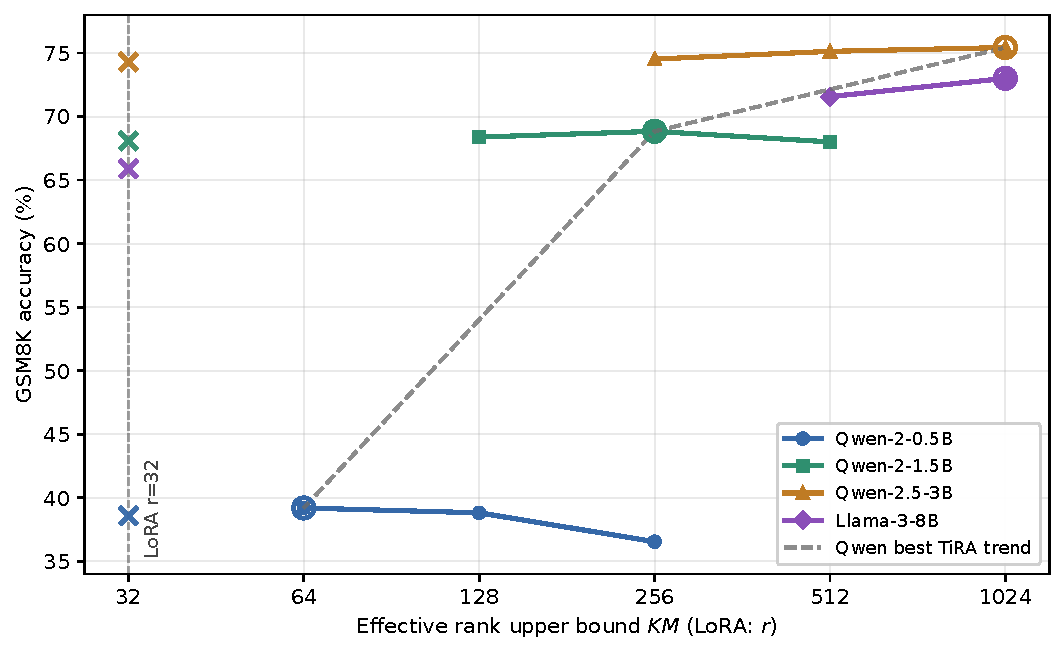
\includegraphics[width=0.88\linewidth]{figures/tira_ablation_m_trend.pdf}
    \caption{固定 $K=32$ 时，Qwen 系列不同规模模型上的分块粒度 $M$ 敏感性分析。横轴表示基座模型的 hidden size，纵轴表示当前配置的总秩上限 $KM$ 与 hidden size 的比例。每个圆点对应一个 TiRA 配置，点内为 GSM8K 准确率，点旁为分块粒度 $M$，颜色表示相对 LoRA（$r=32$）的准确率增减。黑色圆环和虚线标出各模型的最优配置及其随模型规模变化的趋势。}
    \label{fig:ablation_m_trend}
\end{figure}

\paragraph{较大的基座模型更受益于细粒度分块。}
表~\ref{tab:ablation} 显示，在固定 $K=32$、并保持可训练参数量与 LoRA（$r=32$）一致的条件下，不同规模基座模型对分块粒度 $M$ 的偏好存在明显差异。沿 Qwen 系列由小到大观察，最优 $M$ 分别为 2、8 和 32；对应的总秩上限 $KM$ 分别为 64、256 和 1024。若比较总秩上限 $KM$ 与 hidden size 的比例，三者最优配置对应的 $KM$/hidden size 分别为 $64/896=7.1\%$、$256/1536=16.7\%$ 和 $1024/2048=50.0\%$。图~\ref{fig:ablation_m_trend} 进一步可视化了这一趋势，表明随着 hidden size 增大，最优配置对应的 $KM$/hidden size 比例也同步上升，说明较大的基座模型更可能受益于更细粒度的分块结构和更高的适配秩上限。需要强调的是，TiRA 要求 $K\geq M$ 且 $K$ 为 $M$ 的整数倍，因此在本组固定 $K=32$ 的实验中，可考察的最大分块粒度为 $M=32$。表~\ref{tab:ablation} 中 Qwen-2.5-3B 与 Llama-3-8B 的最优结果均出现在这一搜索边界上，因而应理解为当前搜索网格内的最优配置，而非全局最优粒度。尤其是 Llama-3-8B 在边界配置下仍取得最高准确率，提示更大规模模型可能尚未达到可受益分块粒度的上限；继续增大 $M$ 是否能够带来进一步提升，则需要在更高 $K$ 预算下验证。总体而言，分块粒度的最优选择与基座模型规模密切相关，较大模型通常具备更强的高秩扰动承载能力，因而更可能从较高的适配秩上限中获益。

\paragraph{TiRA 的结构优势随基座模型规模增大而扩大。}
在三档 Qwen 模型上，TiRA 的最优配置均优于 LoRA 基线，Qwen-2-0.5B、Qwen-2-1.5B 和 Qwen-2.5-3B 分别提升 $0.61$、$0.76$ 和 $1.14$ 个百分点。进一步纳入 Llama-3-8B 后，该增益扩大至 $6.97$ 个百分点。如图~\ref{fig:best_gain_scale} 所示，最佳 TiRA 配置相对 LoRA（$r=32$）的优势在更大规模模型上更为明显。值得注意的是，随着模型规模增大，可训练参数占比由 $2.33\%$ 降至 $0.70\%$，但其相对增益仍整体保持。这表明，该方法的优势主要来自结构层面的高秩扩展能力，而非参数预算增加。

\begin{figure}[H]
    \centering
    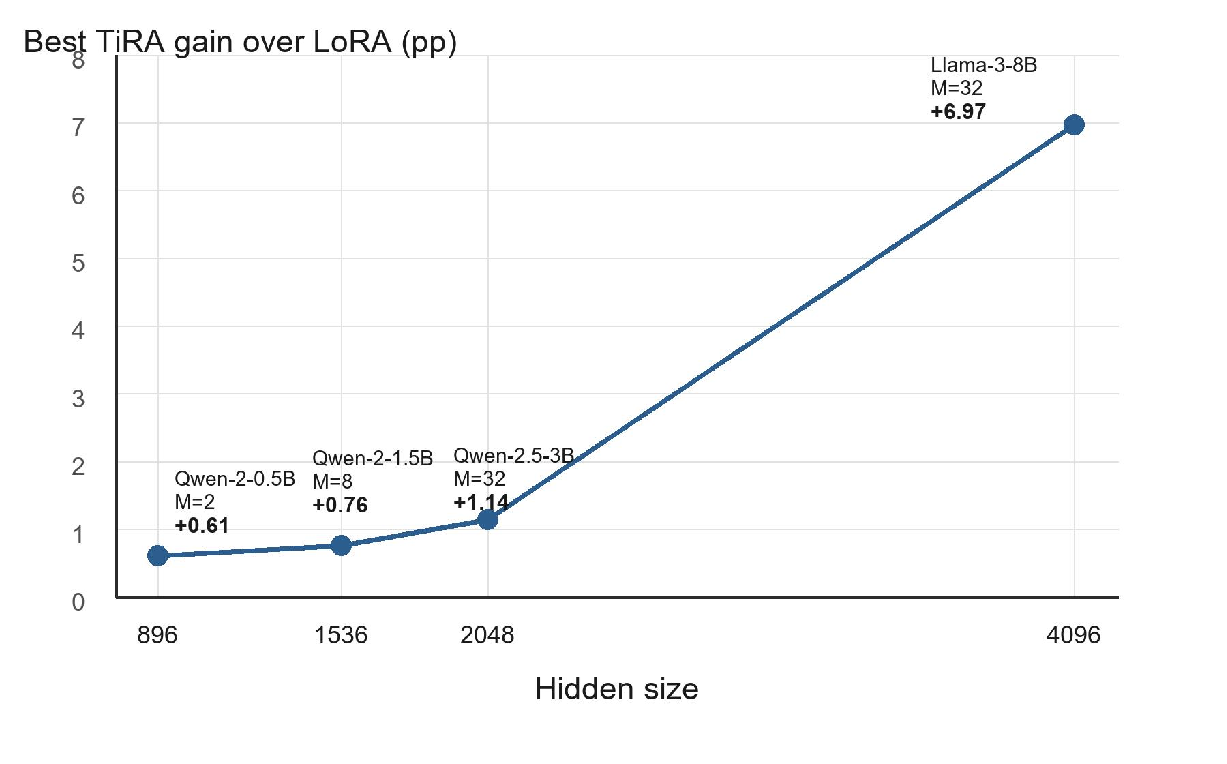
\includegraphics[width=0.82\linewidth]{figures/tira_best_gain_vs_scale.pdf}
    \caption{不同模型规模下最佳 TiRA 配置相对 LoRA（$r=32$）的准确率增益。横轴为 hidden size，纵轴为最佳 TiRA 与 LoRA 的 GSM8K 准确率差值。点旁标注对应模型在当前搜索范围内的最优分块粒度 $M$。}
    \label{fig:best_gain_scale}
\end{figure}

\paragraph{过高分块粒度可能引发秩过载效应。}
TiRA 的性能并不会随分块粒度 $M$ 增大而单调提升。以 Qwen-2-0.5B 为例，当 $M$ 从 2 增大到 4 时准确率已出现下降，继续增大至 $M=8$ 后进一步降至 $36.54\%$，低于 LoRA 基线的 $38.59\%$。Qwen-2-1.5B 也在 $M=16$ 时回落至 $68.01\%$，低于其最优配置 $M=8$ 时的 $68.84\%$。结合前文对分块结构的分析可以看到，增大 $M$ 一方面提高了全局秩上限并扩大了局部更新的覆盖范围，另一方面也会将同等参数预算分散到更多输入、输出通道块之间。当这种分散程度超过当前基座模型规模所能有效承载的范围时，训练过程需要协调过多局部低秩分量，因而难以将其组合为有效的整体更新。本文将这一现象称为“秩过载”效应。这一现象说明，TiRA 的“局部低秩、全局分散”结构先验需要与基座模型的表征空间相匹配。较大模型通常具有更高的 hidden size、更强的参数冗余和更充分的表征空间，任务相关特征也更可能分布在相对分离的子空间中，因此多个局部低秩更新更容易分别作用于不同通道块或特征方向，并在优化过程中形成全局一致的更新。相反，小模型的可调整空间有限；当 $M$ 相对过大时，过多局部分量可能竞争相同或相近的特征通道，使梯度方向冲突和优化耦合增强，从而抵消分块高秩结构可能带来的收益。

\section{结论}

本文提出 TiRA，一种面向大语言模型的分块化高秩参数高效适配方法。TiRA 在保持与 LoRA 相同可训练参数量级的前提下，通过重新组织权重增量矩阵中的可训练参数，突破 LoRA 的全局低秩约束，并形成分块高秩更新结构。同时，TiRA 保留了 LoRA 可合并、无额外推理开销的优势。大量实验表明，在同等参数预算设置下，TiRA 在常识推理、开放域对话生成和数学推理任务上整体优于现有代表性 PEFT 方法；谱分析进一步表明，训练后实测有效秩由 LoRA 的约 32 提升至 TiRA（$M=32,K=32$）的约 757。未来工作将进一步探索 TiRA 在更多模型规模、任务类型和实际应用场景中的表现，并研究分块粒度与模型规模、任务复杂度之间的更一般性匹配规律。

\begin{thebibliography}{99}

\bibitem{hu2022lora}
E. J. Hu, Y. Shen, P. Wallis, Z. Allen-Zhu, Y. Li, S. Wang, L. Wang, and W. Chen, ``LoRA: Low-rank adaptation of large language models,'' in \emph{International Conference on Learning Representations}, 2022.

\bibitem{zhang2023adalora}
Q. Zhang, M. Chen, A. Bukharin, N. Karampatziakis, P. He, Y. Cheng, W. Chen, and T. Zhao, ``AdaLoRA: Adaptive budget allocation for parameter-efficient fine-tuning,'' in \emph{International Conference on Learning Representations}, 2023.

\bibitem{albert2025randlora}
P. Albert, F. Z. Zhang, H. Saratchandran, C. Rodriguez-Opazo, A. van den Hengel, and E. Abbasnejad, ``RandLoRA: Full-rank parameter-efficient fine-tuning of large models,'' \emph{arXiv preprint arXiv:2502.00987}, 2025.

\bibitem{cobbe2021gsm8k}
K. Cobbe, V. Kosaraju, M. Bavarian, M. Chen, H. Jun, L. Kaiser, M. Plappert, J. Tworek, J. Hilton, R. Nakano, C. Hesse, and J. Schulman, ``Training verifiers to solve math word problems,'' \emph{arXiv preprint arXiv:2110.14168}, 2021.

\bibitem{liu2024dora}
S.-Y. Liu, C.-Y. Wang, H. Yin, P. Molchanov, Y.-C. F. Wang, K.-T. Cheng, and M.-H. Chen, ``DoRA: Weight-decomposed low-rank adaptation,'' in \emph{International Conference on Machine Learning}, 2024.

\bibitem{jiang2024mora}
T. Jiang, S. Huang, S. Luo, Z. Zhang, H. Huang, F. Wei, W. Deng, F. Sun, Q. Zhang, D. Wang, and F. Zhuang, ``MoRA: High-rank updating for parameter-efficient fine-tuning,'' \emph{arXiv preprint arXiv:2405.12130}, 2024.

\bibitem{huang2025hira}
Q. Huang, T. Ko, Z. Zhuang, Y. Liu, Y. Wang, M. Hasegawa-Johnson, S. Watanabe, and Z. D. Chen, ``HiRA: Parameter-efficient Hadamard high-rank adaptation for large language models,'' in \emph{International Conference on Learning Representations}, 2025.

\bibitem{li2021prefix}
X. L. Li and P. Liang, ``Prefix-tuning: Optimizing continuous prompts for generation,'' in \emph{Proceedings of ACL-IJCNLP}, 2021, pp. 4582--4597.

\bibitem{lester2021power}
B. Lester, R. Al-Rfou, and N. Constant, ``The power of scale for parameter-efficient prompt tuning,'' in \emph{Proceedings of EMNLP}, 2021, pp. 3045--3059.

\bibitem{xiao2022ptuning}
L. Xiao, K. Ji, and Y. Fu, ``P-tuning v2: Prompt tuning can be comparable to fine-tuning universally across scales,'' \emph{arXiv preprint arXiv:2110.07602}, 2022.

\bibitem{vaswani2017attention}
A. Vaswani, N. Shazeer, N. Parmar, J. Uszkoreit, L. Jones, A. N. Gomez, L. Kaiser, and I. Polosukhin, ``Attention is all you need,'' in \emph{Advances in Neural Information Processing Systems}, vol. 30, 2017.

\bibitem{he2015rectifier}
K. He, X. Zhang, S. Ren, and J. Sun, ``Delving deep into rectifiers: Surpassing human-level performance on ImageNet classification,'' in \emph{Proceedings of ICCV}, 2015, pp. 1026--1034.

\bibitem{hu2023llmadapters}
Z. Hu, L. Wang, Y. Lan, W. Xu, E.-P. Lim, L. Bing, X. Xu, S. Poria, and R. K.-W. Lee, ``LLM-Adapters: An adapter family for parameter-efficient fine-tuning of large language models,'' in \emph{Proceedings of EMNLP}, 2023, pp. 5254--5276.

\bibitem{bisk2019boolq}
Y. Bisk, C. ZelleClark, K. Lee, C. Chang, M. W. Chang, and K. Toutanova, ``BoolQ: Exploring the surprising difficulty of natural yes/no questions,'' in \emph{Proceedings of NAACL-HLT}, 2019, pp. 2924--2936.

\bibitem{bisk2020piqa}
Y. Bisk, R. Zellers, J. Gao, Y. Choi, et al., ``PIQA: Reasoning about physical commonsense in natural language,'' in \emph{Proceedings of AAAI}, vol. 34, no. 05, 2020, pp. 7432--7439.

\bibitem{sap2019socialiqa}
M. Sap, H. Rashkin, D. Chen, R. Le Bras, and Y. Choi, ``Social IQa: Commonsense reasoning about social interactions,'' in \emph{Proceedings of EMNLP-IJCNLP}, 2019, pp. 4463--4473.

\bibitem{zellers2019hellaswag}
R. Zellers, A. Holtzman, Y. Bisk, A. Farhadi, and Y. Choi, ``HellaSwag: Can a machine really finish your sentence?'' in \emph{Proceedings of ACL}, 2019, pp. 4791--4800.

\bibitem{sakaguchi2021winogrande}
K. Sakaguchi, R. L. Bras, C. Bhagavatula, and Y. Choi, ``WinoGrande: An adversarial Winograd schema challenge at scale,'' \emph{Communications of the ACM}, vol. 64, no. 9, pp. 99--106, 2021.

\bibitem{clark2018arc}
P. Clark, I. Cowhey, O. Etzioni, T. Khot, A. Sabharwal, C. Schoenick, and O. Tafjord, ``Think you have solved question answering? Try ARC, the AI2 reasoning challenge,'' \emph{arXiv preprint arXiv:1803.05457}, 2018.

\bibitem{mihaylov2018openbookqa}
T. Mihaylov, P. Clark, T. Khot, and A. Sabharwal, ``Can a suit of armor conduct electricity? A new dataset for open book question answering,'' in \emph{Proceedings of EMNLP}, 2018, pp. 2381--2391.

\bibitem{dinan2019convai2}
E. Dinan, V. Logacheva, V. Malykh, A. H. Miller, K. Shuster, J. Urbanek, D. Kiela, A. Szlam, I. Serban, R. Lowe, S. Prabhumoye, A. W. Black, A. Rudnicky, J. Williams, J. Pineau, M. Burtsev, and J. Weston, ``The second conversational intelligence challenge (ConvAI2),'' in \emph{The NeurIPS'18 Competition: From Machine Learning to Intelligent Conversations}. Springer, 2019, pp. 187--208.

\bibitem{yu2024metamath}
L. Yu, W. Jiang, H. Shi, J. Yu, Z. Liu, Y. Zhang, J. T. Kwok, Z. Li, A. Weller, and W. Liu, ``MetaMath: Bootstrap your own mathematical questions for large language models,'' in \emph{International Conference on Learning Representations}, 2024.

\bibitem{papineni2002bleu}
K. Papineni, S. Roukos, T. Ward, and W.-J. Zhu, ``BLEU: A method for automatic evaluation of machine translation,'' in \emph{Proceedings of ACL}, 2002, pp. 311--318.

\bibitem{banerjee2005meteor}
S. Banerjee and A. Lavie, ``METEOR: An automatic metric for MT evaluation with improved correlation with human judgments,'' in \emph{Proceedings of the ACL Workshop on Intrinsic and Extrinsic Evaluation Measures for Machine Translation and/or Summarization}, 2005, pp. 65--72.

\bibitem{lin2004rouge}
C.-Y. Lin, ``ROUGE: A package for automatic evaluation of summaries,'' in \emph{Text Summarization Branches Out}, 2004, pp. 74--81.

\bibitem{zhang2019bertscore}
T. Zhang, V. Kishore, F. Wu, K. Q. Weinberger, and Y. Artzi, ``BERTScore: Evaluating text generation with BERT,'' \emph{arXiv preprint arXiv:1904.09675}, 2019.

\bibitem{touvron2023llama2}
H. Touvron, L. Martin, K. Stone, P. Albert, A. Almahairi, Y. Babaei, N. Bashlykov, S. Batra, P. Bhargava, S. Bhosale, et al., ``Llama 2: Open foundation and fine-tuned chat models,'' \emph{arXiv preprint arXiv:2307.09288}, 2023.

\bibitem{grattafiori2024llama3}
A. Grattafiori, A. Dubey, A. Jauhri, A. Pandey, A. Kadian, A. Al-Dahle, A. Letman, A. Mathur, A. Schelten, A. Vaughan, et al., ``The Llama 3 herd of models,'' \emph{arXiv preprint arXiv:2407.21783}, 2024.

\bibitem{yang2024qwen2}
A. Yang, B. Yang, B. Hui, B. Zheng, B. Yu, C. Zhou, C. Li, C. Li, D. Liu, F. Huang, et al., ``Qwen2 technical report,'' \emph{arXiv preprint arXiv:2407.10671}, 2024.

\bibitem{yang2024qwen25}
A. Yang, B. Yang, B. Zhang, B. Hui, B. Zheng, B. Yu, C. Li, D. Liu, F. Huang, H. Wei, et al., ``Qwen2.5 technical report,'' \emph{arXiv preprint arXiv:2412.15115}, 2024.

\end{thebibliography}

\appendix

\section{TiRA 构造示例}

\subsection{$K=M=3$ 的分块构造}
\label{app:k3m3}

以 $K=M=3$ 为例，三个适配组分别占据三条互异的循环移位对角线，其稀疏增量矩阵可写为
\begin{equation}
\Delta W_0=
\begin{bmatrix}
C_{0,0} & 0 & 0\\
0 & C_{0,1} & 0\\
0 & 0 & C_{0,2}
\end{bmatrix},\quad
\Delta W_1=
\begin{bmatrix}
0 & C_{1,0} & 0\\
0 & 0 & C_{1,1}\\
C_{1,2} & 0 & 0
\end{bmatrix},\quad
\Delta W_2=
\begin{bmatrix}
0 & 0 & C_{2,0}\\
C_{2,1} & 0 & 0\\
0 & C_{2,2} & 0
\end{bmatrix}
\end{equation}
其中 $C_{k,m}\in\R^{(d_{\mathrm{out}}/M)\times(d_{\mathrm{in}}/M)}$ 为第 $k$ 个适配组沿其循环移位对角线的第 $m$ 个秩为 1 的外积子块。三者沿错位块对角线互补分布，叠加后在全部 $3\times3$ 个块位置形成非零子块：
\begin{equation}
\DeltaW=
\begin{bmatrix}
C_{0,0} & C_{1,0} & C_{2,0}\\
C_{2,1} & C_{0,1} & C_{1,1}\\
C_{1,2} & C_{2,2} & C_{0,2}
\end{bmatrix}
\end{equation}

\subsection{多稀疏 LoRA 专家适配示例}
\label{app:sparse_expert}

当 $d_{\mathrm{in}}=9$、$d_{\mathrm{out}}=9$ 且 $r=3$ 时，稀疏 LoRA 专家适配的增量矩阵可写为如下形式。

第一组为无错位分组，对应 $k=0$：
\[
\resizebox{\linewidth}{!}{$\displaystyle
\mathbf{B}_0 \mathbf{A}_0^\top =
\begin{bmatrix}
a_1 & 0 & 0 \\ 0 & a_2 & 0 \\ 0 & 0 & a_3 \\
b_1 & 0 & 0 \\ 0 & b_2 & 0 \\ 0 & 0 & b_3 \\
c_1 & 0 & 0 \\ 0 & c_2 & 0 \\ 0 & 0 & c_3
\end{bmatrix}
\begin{bmatrix}
m_1 & 0 & 0 & n_1 & 0 & 0 & o_1 & 0 & 0 \\
0 & m_2 & 0 & 0 & n_2 & 0 & 0 & o_2 & 0 \\
0 & 0 & m_3 & 0 & 0 & n_3 & 0 & 0 & o_3
\end{bmatrix}
=
\begin{bmatrix}
a_1 m_1 & 0 & 0 & a_1 n_1 & 0 & 0 & a_1 o_1 & 0 & 0 \\
0 & a_2 m_2 & 0 & 0 & a_2 n_2 & 0 & 0 & a_2 o_2 & 0 \\
0 & 0 & a_3 m_3 & 0 & 0 & a_3 n_3 & 0 & 0 & a_3 o_3 \\
b_1 m_1 & 0 & 0 & b_1 n_1 & 0 & 0 & b_1 o_1 & 0 & 0 \\
0 & b_2 m_2 & 0 & 0 & b_2 n_2 & 0 & 0 & b_2 o_2 & 0 \\
0 & 0 & b_3 m_3 & 0 & 0 & b_3 n_3 & 0 & 0 & b_3 o_3 \\
c_1 m_1 & 0 & 0 & c_1 n_1 & 0 & 0 & c_1 o_1 & 0 & 0 \\
0 & c_2 m_2 & 0 & 0 & c_2 n_2 & 0 & 0 & c_2 o_2 & 0 \\
0 & 0 & c_3 m_3 & 0 & 0 & c_3 n_3 & 0 & 0 & c_3 o_3
\end{bmatrix}
$}
\]

第二组沿列方向循环偏移 1，对应 $k=1$：
\[
\resizebox{\linewidth}{!}{$\displaystyle
\mathbf{B}_1 \mathbf{A}_1^\top =
\begin{bmatrix}
e_1 & 0 & 0 \\ 0 & e_2 & 0 \\ 0 & 0 & e_3 \\
f_1 & 0 & 0 \\ 0 & f_2 & 0 \\ 0 & 0 & f_3 \\
g_1 & 0 & 0 \\ 0 & g_2 & 0 \\ 0 & 0 & g_3
\end{bmatrix}
\begin{bmatrix}
0 & q_2 & 0 & 0 & r_2 & 0 & 0 & s_2 & 0 \\
0 & 0 & q_3 & 0 & 0 & r_3 & 0 & 0 & s_3 \\
q_1 & 0 & 0 & r_1 & 0 & 0 & s_1 & 0 & 0
\end{bmatrix}
=
\begin{bmatrix}
0 & e_1 q_2 & 0 & 0 & e_1 r_2 & 0 & 0 & e_1 s_2 & 0 \\
0 & 0 & e_2 q_3 & 0 & 0 & e_2 r_3 & 0 & 0 & e_2 s_3 \\
e_3 q_1 & 0 & 0 & e_3 r_1 & 0 & 0 & e_3 s_1 & 0 & 0 \\
0 & f_1 q_2 & 0 & 0 & f_1 r_2 & 0 & 0 & f_1 s_2 & 0 \\
0 & 0 & f_2 q_3 & 0 & 0 & f_2 r_3 & 0 & 0 & f_2 s_3 \\
f_3 q_1 & 0 & 0 & f_3 r_1 & 0 & 0 & f_3 s_1 & 0 & 0 \\
0 & g_1 q_2 & 0 & 0 & g_1 r_2 & 0 & 0 & g_1 s_2 & 0 \\
0 & 0 & g_2 q_3 & 0 & 0 & g_2 r_3 & 0 & 0 & g_2 s_3 \\
g_3 q_1 & 0 & 0 & g_3 r_1 & 0 & 0 & g_3 s_1 & 0 & 0
\end{bmatrix}
$}
\]

第三组沿列方向循环偏移 2，对应 $k=2$：
\[
\resizebox{\linewidth}{!}{$\displaystyle
\mathbf{B}_2 \mathbf{A}_2^\top =
\begin{bmatrix}
i_1 & 0 & 0 \\ 0 & i_2 & 0 \\ 0 & 0 & i_3 \\
j_1 & 0 & 0 \\ 0 & j_2 & 0 \\ 0 & 0 & j_3 \\
k_1 & 0 & 0 \\ 0 & k_2 & 0 \\ 0 & 0 & k_3
\end{bmatrix}
\begin{bmatrix}
0 & 0 & u_3 & 0 & 0 & v_3 & 0 & 0 & w_3 \\
u_1 & 0 & 0 & v_1 & 0 & 0 & w_1 & 0 & 0 \\
0 & u_2 & 0 & 0 & v_2 & 0 & 0 & w_2 & 0
\end{bmatrix}
=
\begin{bmatrix}
0 & 0 & i_1 u_3 & 0 & 0 & i_1 v_3 & 0 & 0 & i_1 w_3 \\
i_2 u_1 & 0 & 0 & i_2 v_1 & 0 & 0 & i_2 w_1 & 0 & 0 \\
0 & i_3 u_2 & 0 & 0 & i_3 v_2 & 0 & 0 & i_3 w_2 & 0 \\
0 & 0 & j_1 u_3 & 0 & 0 & j_1 v_3 & 0 & 0 & j_1 w_3 \\
j_2 u_1 & 0 & 0 & j_2 v_1 & 0 & 0 & j_2 w_1 & 0 & 0 \\
0 & j_3 u_2 & 0 & 0 & j_3 v_2 & 0 & 0 & j_3 w_2 & 0 \\
0 & 0 & k_1 u_3 & 0 & 0 & k_1 v_3 & 0 & 0 & k_1 w_3 \\
k_2 u_1 & 0 & 0 & k_2 v_1 & 0 & 0 & k_2 w_1 & 0 & 0 \\
0 & k_3 u_2 & 0 & 0 & k_3 v_2 & 0 & 0 & k_3 w_2 & 0
\end{bmatrix}
$}
\]

三组叠加后得到完整的增量矩阵：
\[
\resizebox{\linewidth}{!}{$\displaystyle
\Delta W_{\text{expert}}
= \frac{\alpha}{K}\left(\mathbf{B}_0 \mathbf{A}_0^\top+\mathbf{B}_1 \mathbf{A}_1^\top+\mathbf{B}_2 \mathbf{A}_2^\top\right)
= \frac{\alpha}{K}
\begin{bmatrix}
a_1 m_1 & e_1 q_2 & i_1 u_3 & a_1 n_1 & e_1 r_2 & i_1 v_3 & a_1 o_1 & e_1 s_2 & i_1 w_3 \\
i_2 u_1 & a_2 m_2 & e_2 q_3 & i_2 v_1 & a_2 n_2 & e_2 r_3 & i_2 w_1 & a_2 o_2 & e_2 s_3 \\
e_3 q_1 & i_3 u_2 & a_3 m_3 & e_3 r_1 & i_3 v_2 & a_3 n_3 & e_3 s_1 & i_3 w_2 & a_3 o_3 \\
b_1 m_1 & f_1 q_2 & j_1 u_3 & b_1 n_1 & f_1 r_2 & j_1 v_3 & b_1 o_1 & f_1 s_2 & j_1 w_3 \\
j_2 u_1 & b_2 m_2 & f_2 q_3 & j_2 v_1 & b_2 n_2 & f_2 r_3 & j_2 w_1 & b_2 o_2 & f_2 s_3 \\
f_3 q_1 & j_3 u_2 & b_3 m_3 & f_3 r_1 & j_3 v_2 & b_3 n_3 & f_3 s_1 & j_3 w_2 & b_3 o_3 \\
c_1 m_1 & g_1 q_2 & k_1 u_3 & c_1 n_1 & g_1 r_2 & k_1 v_3 & c_1 o_1 & g_1 s_2 & k_1 w_3 \\
k_2 u_1 & c_2 m_2 & g_2 q_3 & k_2 v_1 & c_2 n_2 & g_2 r_3 & k_2 w_1 & c_2 o_2 & g_2 s_3 \\
g_3 q_1 & k_3 u_2 & c_3 m_3 & g_3 r_1 & k_3 v_2 & c_3 n_3 & g_3 s_1 & k_3 w_2 & c_3 o_3
\end{bmatrix}
$}
\]

\subsection{$M=3,K=6$ 的多层叠加构造}
\label{app:m3k6}

以 $M=3,K=6$（$L=2$）为例，第 0 条斜带由第 0 组和第 3 组共同产生，第 1 条斜带由第 1 组和第 4 组共同产生，第 2 条斜带由第 2 组和第 5 组共同产生。同一斜带上的对应块位置进行求和累加，因此总增量矩阵为
\begin{equation}
\DeltaW=
\begin{bmatrix}
C_{0,0}+C_{3,0} & C_{1,0}+C_{4,0} & C_{2,0}+C_{5,0}\\
C_{2,1}+C_{5,1} & C_{0,1}+C_{3,1} & C_{1,1}+C_{4,1}\\
C_{1,2}+C_{4,2} & C_{2,2}+C_{5,2} & C_{0,2}+C_{3,2}
\end{bmatrix}
\end{equation}
此时每个单元块由两个独立的秩为 1 的外积叠加形成，块内秩上限由 1 提升至 2。

\section{超参数设置}

\subsection{LoRA 超参数设置}
\label{app:lora_hyperparams}

\begin{table}[H]
\centering
\caption{任务复杂度与 LoRA 秩需求关系验证实验的 LoRA 超参数设置。}
\begin{tabular}{ll}
\toprule
Hyperparameter & Value \\
\midrule
Base Model & Qwen-2-1.5B \\
Method & LoRA \\
Datasets & GSM8K-Easy, GSM8K-Challenge \\
LoRA Rank ($r$) & 8, 16, 32, 64, 128 \\
LoRA Alpha ($\alpha$) & 8, 16, 32, 64, 128 \\
LoRA Dropout & 0.05 \\
Learning Rate & $1\times10^{-4}$ \\
Epochs & 2 \\
Batch Size & 160 \\
Warmup & 100 steps \\
Weight Decay & 0 \\
Target Modules & q\_proj, k\_proj, v\_proj, up\_proj, down\_proj \\
Evaluation Steps & Every 2 steps \\
\bottomrule
\end{tabular}
\end{table}

\subsection{TiRA 超参数设置}
\label{app:tira_hyperparams}

\begin{table}[H]
\centering
\caption{主要实验中的 TiRA 超参数设置。}
\begin{tabular}{ll}
\toprule
Hyperparameter & Value \\
\midrule
Optimizer & AdamW \\
Weight Decay & 0 \\
Warmup & 100 steps \\
Batch Size & 32 \\
Target Modules & q\_proj, k\_proj, v\_proj, up\_proj, down\_proj \\
Evaluation Steps & Every 80 steps \\
\midrule
Commonsense Base Models & Llama-2-7B, Llama-3-8B \\
Commonsense $K,M$ & 32, 32 \\
Commonsense Learning Rate & $2\times10^{-4}$ \\
Commonsense Epochs & 2 \\
\midrule
Dialogue Base Model & Llama-3-8B \\
Dialogue $K,M$ & 32, 32 \\
Dialogue Learning Rate & $2\times10^{-5}$ \\
Dialogue Epochs & 1 \\
\midrule
Math Base Model & Llama-3-8B \\
Math $K,M$ & 32, 16/32 \\
Math Learning Rate & $4\times10^{-5}$ \\
Math Epochs & 2 \\
\bottomrule
\end{tabular}
\end{table}

\subsection{超参数设置}
\label{app:ablation_hyperparams}

\begin{table}[H]
\centering
\caption{分块粒度 M 对 TiRA 适配性能影响的实验超参数设置。}
\begin{tabular}{ll}
\toprule
Hyperparameter & Value \\
\midrule
Dataset & MetaMath \\
Epochs & 2 \\
Batch Size & 32 \\
Warmup & 100 steps \\
Weight Decay & 0 \\
Target Modules & q\_proj, k\_proj, v\_proj, up\_proj, down\_proj \\
Evaluation Steps & Every 100 steps \\
\midrule
LoRA Rank/Alpha & 32/32 \\
LoRA Dropout & 0 \\
\midrule
TiRA Qwen-2-0.5B & $K=32$, $M\in\{2,4,8\}$, Learning Rate $1\times10^{-4}$ \\
TiRA Qwen-2-1.5B & $K=32$, $M\in\{2,4,8,16\}$, Learning Rate $7\times10^{-5}$ \\
TiRA Qwen-2.5-3B & $K=32$, $M\in\{8,16,32\}$, Learning Rate $5\times10^{-5}$ \\
\bottomrule
\end{tabular}
\end{table}

\end{document}
